\documentclass[11pt,letterpaper]{article}
\oddsidemargin 0in
\evensidemargin 0in
\textwidth 6.5in
\topmargin -0.5in
\textheight 9.0in
\usepackage{hyperref}
\usepackage{mathptmx}
\usepackage{graphicx}
\usepackage{natbib} % for references
\usepackage{amsmath}
\usepackage{subfig}
\usepackage{multirow}
\usepackage[usenames,dvipsnames]{xcolor}
\usepackage{float}
\newcommand{\blue}[1]{\textcolor{RoyalBlue}{#1}}
\newcommand{\fillme}[1]{\blue{\texttt{[Insert #1]}}}
\newcommand{\instructions}[1]{\blue{\textit{#1}}}
% uncomment the next two lines if you want the instructions to disappear.
%\renewcommand{\instructions}[1]{}
%\renewcommand{\fillme}[1]{}

\begin{document}

\title{STAT542 Class Project: Kaggle Biometric Accelerometer Data Competition}
\author{Wenzhao Xu(wxu15),Haoyan Cai(hcai6)}
\maketitle





\begin{abstract}
We consider multi-class classification and binary classification on the Kaggle Biometric Accelerometer Data to tell whether one sequence in test set belongs to the proposed device Id. It turned out that multi-class version is less efficient and not as accurate than one-all binary classifications. We further experimented on several learning algorithms including K Nearest Neighbour, Support Vector Machine, Linear Discriminant Analysis, Lasso, Logistic and Random Forest. Random Forest provide the best performance of 78.1\% without using data leakage.

\end{abstract}


\section{Introduction} 
\label{sec:introduction}
\paragraph{} Since everyone moves differently and accelerometers are fast becoming ubiquitous, this Kaggle competition is designed to investigate the feasibility of using accelerometer data as a biometric for identifying users of mobile devices. Accelerometer data is collected from several hundred users over a period of several months during normal device usage. 
 The train data contain X,Y,Z axis acceleration values from 387 devices and testing data set consists of 90024 testing sequences. Samples in the training set are labeled with the unique device from which the data was collected but each test sequence comes with a proposed device Id. The goal is to judge whether the claimed device is the true device that produces the test sequence. 
	
 

\section{Background}
\label{sec:background}
\paragraph{} An accelerometer is an electromechanical device that will measure acceleration forces. These forces may be static, like the constant force of gravity pulling at your feet, or they could be dynamic - caused by moving or vibrating the accelerometer. By measuring the amount of static acceleration due to gravity, you can find out the angle the device is tilted at with respect to the earth. By sensing the amount of dynamic acceleration, you can analyze the way the device is moving. At first, measuring tilt and acceleration doesn't seem all that exciting. However, engineers have come up with many ways to make really useful products with them. In the computing world, IBM and Apple have recently started using accelerometers in their laptops to protect hard drives from damage. If you accidentally drop the laptop, the accelerometer detects the sudden freefall, and switches the hard drive off so the heads don't crash on the platters. In a similar fashion, accelerometers are the industry standard way of detecting car crashes and deploying airbags at just the right time.\\

The main difficulties in this project are: (1) Data have outliers and gaps (i.e. the sampling time interval is not constant so that two sampling points might have very large time interval); (2) Expressive feature extractions; (3) Treat it as a multi-label classificationn problem or as a 0-1 classification problem by some label creating methods (4) Given the large scale of data, efficient algorithms is in demand.

\section{Task and Data Preprocessing}
\label{sec:taskAndData}

\subsection{The Task}
\label{sec:task}
\paragraph{User Matching} Since the data is equally split into training and test sets. It is reasonable to justify whether a test sequence comes from the proposed device using models learnt from training sets. Whether we took a multi-classification or binary classification approach remains to be seen from experiments we will conduct. We are prone to use binary classification because it is less expensive and more intuitive towards this particular matching task.
\subsection{Data Preprocessing}
\label{sec:data}
We need to preprocess data in order to turn the data into usable forms. It is first imported into R by "ff" packages (or by SQL database). Preprocessing procedures include: splitting,resampling and smoothing. Figure 1 shows an brief of how data is pre-processed.
\begin{figure}
	\centering
	\subfloat[Splitting]{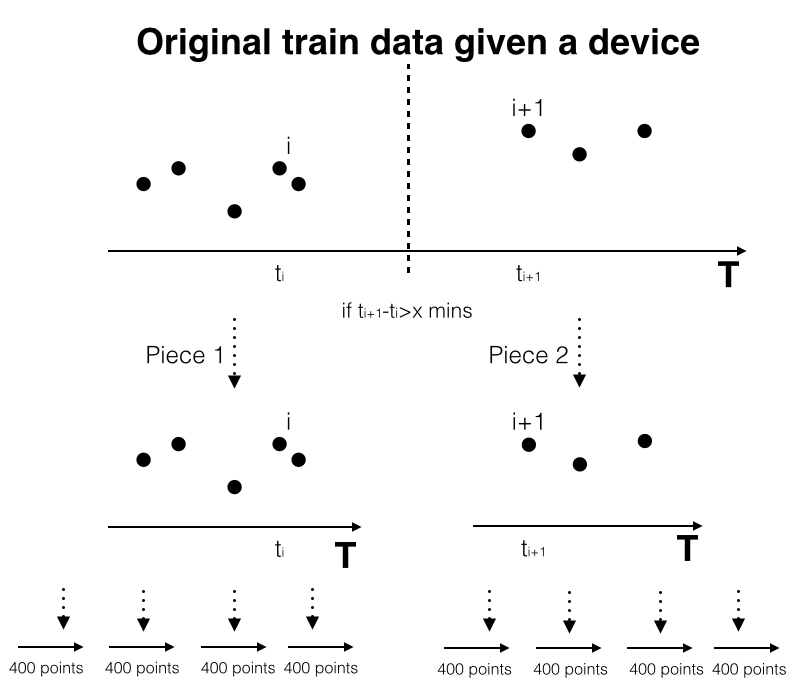
\includegraphics[width=0.6\textwidth]{split.png}}
	\subfloat[Resampling]{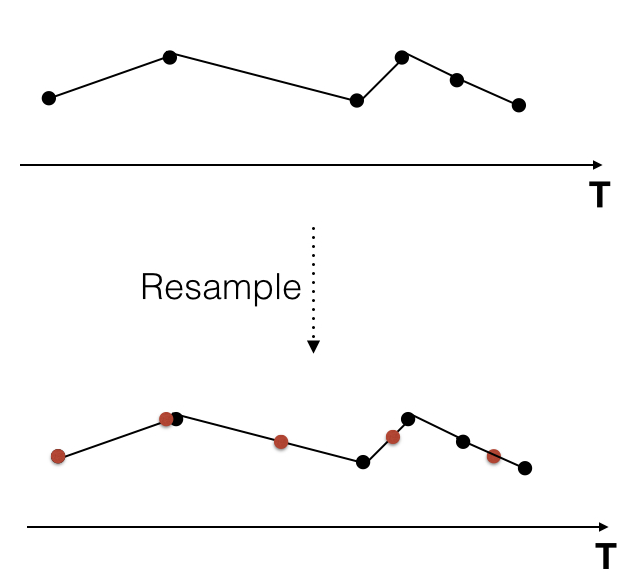
\includegraphics[width=0.4\textwidth]{resampling.png}}
	\caption{Splitting and Resampling Steps}
\end{figure}

\subsubsection{Splitting}
		\paragraph{} It is found that the training data of a given device don’t have a constant sampling frequency, that is, the time interval of sampling poitns are not the same. This might be due to users’ manually switching off device or the way Android OS deal with accelerometer sensors. So the whole training data might have large gaps in time. In order to deal with this, we first calcuate the sampling time intervals. If the time interval is larger that 2 minutes, we split the training data into two data pieces at this point. After the data is divided into several pieces, we further divide each pieces into smaller sequences, each sequence has 300 raw data points (we also test on 400 data points). At the end of this step, the training data from 387 devices are splited into almost 70000 sequences. This step is shown in Figure 1(a). In addition, for test data, similar splitting method is used. If the time interval in one test sequence is larger than 3 minutes, we divide the test sequence into 2 parts and discard the part with less data points.

		\subsubsection{Resampling}
		\paragraph{} In splitting step, we split the train data into sequences. However, in each sequence, the sampling frequencies are not always the same. Some might be 200 ms other others might be around 100ms. Such inconsistance makes it very hard for further analysis, especially for frequency analysis. So we do a resample step. A constant sampling time is set based on the initial sampling time and the median value of original sampling intervals. Here median value is used to eliminate the influence of sampling interval outliers. Then, on the new sampling time, the resampled acceralation value is calculated by linear interpolation based on two nearest sampling points. In Figure 1(b), the brown points are the new data points based on interpolation. 
		\subsubsection{Smoothing}
		\paragraph{} Train data have noises such as large spikes. Smoothing it will result in better performance in pattern recognition. So a 5-point moving average algorithm is then used to smooth the data. 5-point moving average is also used in other literatures. Figure 2 shows the a piece of data before and after resampling and smoothing steps.
		% subsection idea (end)
		\begin{figure}
			\centering
			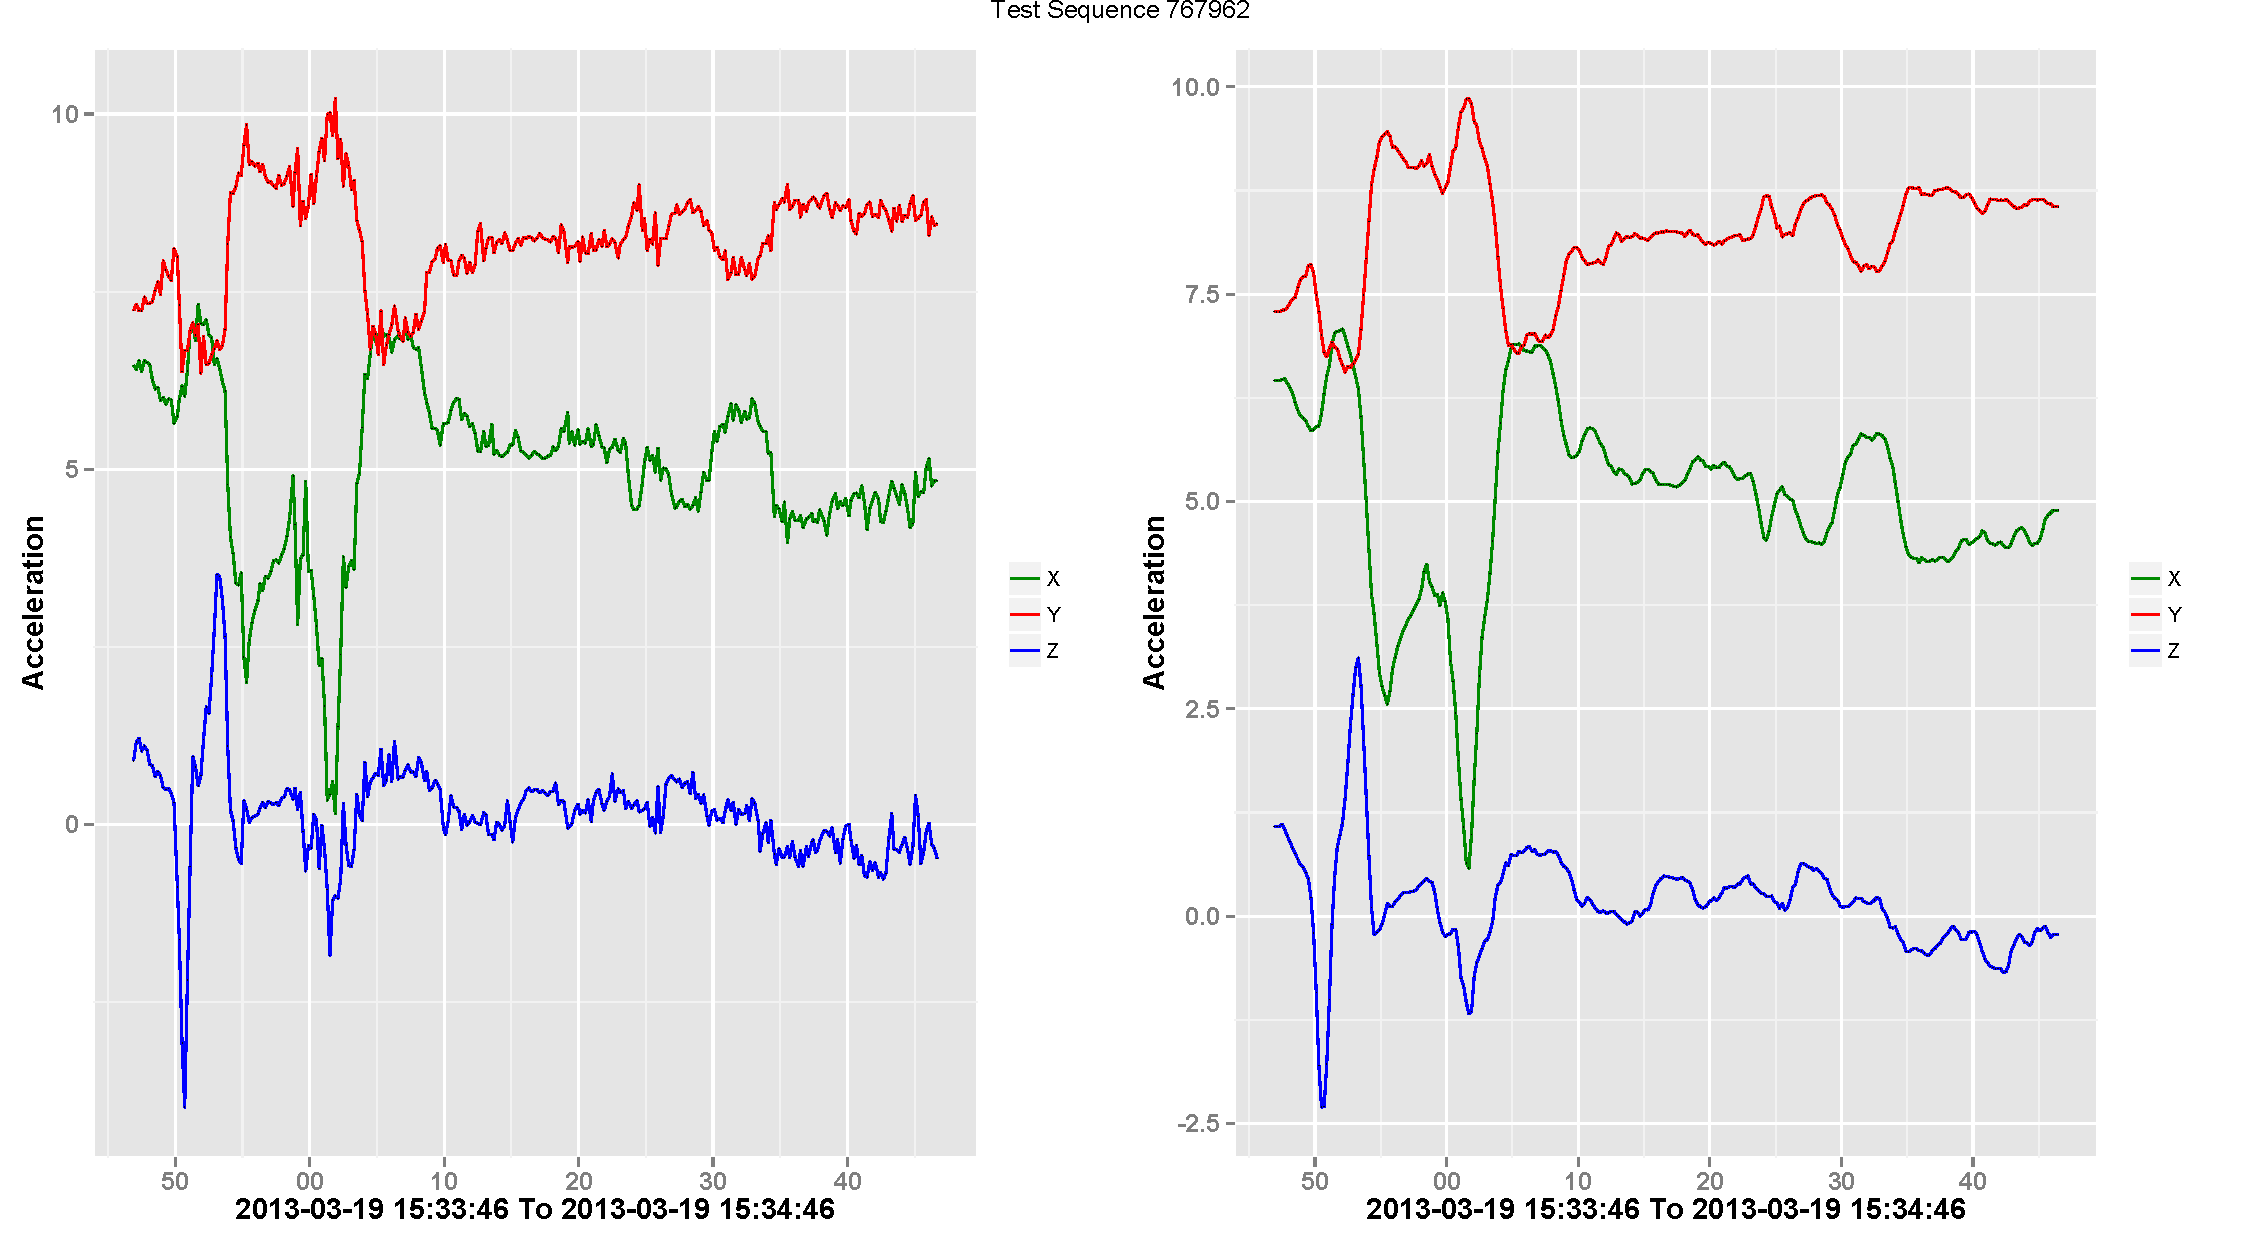
\includegraphics[width=0.9\textwidth]{Rplot.pdf}
			\caption{Comparison before and after resampling and smoothing}
		\end{figure}
	

\section{The Models}
\label{sec:models}
\paragraph{} We consider this a classification problem, multi-classification or binary classification. Correspondingly, the training data is constructed in different manners according to the approach we take. In multi-classification the label space is the set of 387 devices. So most algorithms would end up inefficient to train on our experiment laptop (Macbook Pro i7 with 8G of RAM). While for binary classification, we only need to tell whether a sequence comes from the proposed device id. And this task is simpler.

\subsection{Baseline Models}
\label{sec:baseline-models}
Base line model of this problem is given by Kaggle, a KNN classifier that provide an accuracy of approximately 50\% on the 90024 test sequences. Kaggle did not release the algorithm but we believe they are taking a similar approach as we will discuss later. Besides, we tried submitting all 0 or all 1 classification to the evaluators and both times, we got 50\%, which means the original test set has equal number of positive examples and negative examples, this is an important factor to consider for constructing training data in the following learning algorithms.




\subsection{Proposed Model(s)}
\label{sec:proposed-models}
In this section, we brief discuss the learning algorithms we use in our experiments, they fall into two categories multi-classification and binary classification.
\paragraph {Multi-classification}
Many learning techniques could be modified to use for multi-classification. We take K nearest neighbour as a representative because it is an intuitive techniques (distance similarity) for this particular task and it is not as expensive as other learning methods.
Based on the processed data and extracted features, for each test sequence, it finds its nearest neighbour in train sequences and assign the majority label to this sequence. This method considers the whole label space (387) and it's non-trivial to do supervised kNN feature extraction.
\paragraph {Binary classification}
We instead formulate this problem as a one-all binary classification problem, i.e. we need to train 387 binary classifiers in advance and apply one of them onto test sequence depending on the proposed device Id. Specifically, for each device $i$, train a classifier $i$ that is used to classify all the test sequence with $i$ as the claimed Id. Now we briefly explain the learning algorithms in our experiments.
\begin{itemize}
\item Support Vector Machine: This is the only large margin classifier we consider in our example. We experimented on different feature set and different kernel methods to know whether kernel method is superior to non-kernel method on this data set.
\item Linear Discriminant Analysis: LDA is a common technique used to find a linear combination of features that could characterize or seperates two or more classes. The resulting combination is used a classifier. In our task, although it is not of our major concern to study the linear combination, we would still use the classifier.
\item Logistic Regression: As a log-linear classifier, it is another commonly used model, it is very easy to generalize to multi-classification by probability modeling, widely known as max entropy classifer.
\item Random Forest: Random Forest is to use bootstrap strategy to generate a large number of trees. The parameters in random forest are the default values in R package, that is, the number of trees are 500 and the number of features that are randomly selected are $\sqrt{p}$.
\item Lasso regression: We also tried Lasso as a representative for shrinkage mdoel.
\end{itemize} 


\section{Experiments}
\label{sec:experiments}

\subsection{Experimental setup}
\label{sec:experimental-setup}
\paragraph{Feature extraction}
In this section, we illustrate our feature extraction methods.
First, the total acceralation value is calculated by $A=\sqrt{(a_x^2+a_y^2+a_z^2)}$ and added as a new time series. Based on literature research, 5 kind of features are extracted from the raw data. The first is mean and variance. The second is the correlation. The third one is Fourier frequency analysis, the forth is the average time (transformed to hours) and the last is sampling frequency. As shown in table 1, we extract 21 features and the importance of features will be studied later.
		\begin{table}
			\centering
			\caption{Feature Selection}
			\begin{tabular}{p{3cm}|p{6cm}|p{4cm}}
			Kind & Description & Physical Meanings \\ \hline
			1.Mean and Variance (8 features) & Mean and variance of acceleration values in each axis as well as the total accerlation $A$ & The habbit of how user put their cellphones and the strength of their activities \\ \hline
			2.Covariance (cov) (3 features) & the covariance coefficients between x and y, x and z, and y and z axis. & The users features when doing activities \\ \hline
			3.Frequency Features (8 features) & The mean value of the first 5 dominant frequencies (frequencies with highest amplitude) and mean value of energy in these frequencies & Users walking features.\\ \hline
			4.Time (1 feature) & mean time of day & Activity patterns are different for different users at different time of the day.\\ \hline
			5.Device sampling frequency (1 feature) & sampling frequency of data & Same mobile hardware collects accerlerometer data at same frequencies.
			\end{tabular}
		\end{table}
\paragraph{Training data construction}
We formulate this task as a binary classification problem, so we need to construct supervised information in order to learn these classifiers. For each device, we have a classifier so there are totally 387 classifiers. We construct our training data in the following way.
\begin{enumerate}
\item For each device in training data, do the splitting, resampling and smoothing to get small training sequences that has a size comparable to approximately 300 points.
\item Construct positive examples: For a classifier of device $i$, label the training sequencies from device $i$ as 1 to form positive samples.
\item Construct negative examples: For a classifier of device $i$, sample and label the training sequencies from device other than $i$ as 0 to form negative samples.
\item Train each classifier with the new formed training data consist of positive and negative samples. Experiments show that when we have a balanced design, i.e. size of positive and negative examples equal, we have the best performance on test data.
\end{enumerate}

\subsection{Experimental results}
\label{sec:experimental-results}
	
In table 2, We have set the cases (parameter set) that we use to conduct experiments. Case 0 is the baseline scenario. Case 1 reduces the features to the basic means and variances. Case 2 add sampling frequencies to the feature space. Case 3 increase the negative sampling size and Case 4 increase the average size of each data pieces.
	
	\begin{table}
		\centering
		\caption{Case Setting}
		\begin{tabular}{c|c|c|c|c}
			Case No & Splitting Size & Feature Selection & Negative Size/ Positive Size \\ \hline
			0 & 300 & Feature 1,2,3,4 & 1 \\
			1 & 300 & Feature 1,2     & 1  \\
			2 & 300 & Feature 1,2,3,4,5 & 1 \\
			3 & 300 & Feature 1,2,3,4 & 5  \\
			4 & 400 & Feature 1,2,3,4 & 1 \\
		\end{tabular}
	\end{table}

We summarize the results in table 3 and table 4. The first two knn methods (knn-1(M) and knn-5(M)) are multi-label KNN classification with k as 1 and 5 respectively. The rest methods are 0-1 classification methods. The training error are calculated by cross-validation (in KNN method), out of bag error (in random forest) or error on training data (in other methods). And the prediction results are uploaded to kaggle website to see the prediction results. 


	\begin{table}
	\centering
	\caption{Accuracy on training data}
	\begin{tabular}{|c|c|c|c|c|c|c|c|c|c|}
	\hline
	CASE NO	& knn-1(M)	& knn-5(M)	& svm-Gaussian & svm-linear & rf	& lda	& lasso &	logit	& knn-5 \\ \hline
0	& 0.584	 & 0.556	& 0.952 &	0.899	& 0.907	& 0.875 &	0.863	& 0.904 & 0.667 \\ \hline
1	& 0.405	 & 0.420	& 0.925	& 0.825	& 0.861	& 0.802	& 0.799	& 0.834	& 0.772 \\ \hline
2	& 0.627	& 0.600	& 0.957	& 0.910	& 0.936	& 0.888	& 0.878	& 0.918	& 0.735 \\ \hline
3	& 0.582	& 0.557	& 0.948	& 0.908	& 0.941	& 0.888	& 0.900	& 0.913	& 0.837 \\ \hline
4	& 0.565	& 0.543	& 0.952	& 0.908	& 0.892	& 0.891	& 0.873	& 0.919	& 0.647 \\ \hline
	\end{tabular}
	\end{table}

	\begin{table}
	\centering
	\caption{Accuracy on test data(submitted to Kaggle)}
	\begin{tabular}{|c|c|c|c|c|c|c|c|c|c|}
	\hline
	CASE NO	& knn-1(M)	& knn-5(M)	& svm-Gaussian & svm-linear	& rf	& lda	& lasso &	logit	& knn-5 \\ \hline
0	& 0.640 & 0.640	& 0.763 &	0.701	& 0.781	& 0.672 &	0.697	& 0.678 & 0.608 \\ \hline
1	& 0.631	 & 0.630	& 0.770	& 0.677	& 0.781	& 0.657	& 0.668	& 0.672	& 0.677 \\ \hline
2	& 0.665 & 0.665	& 0.769	& 0.713	& 0.812	& 0.668	& 0.699	& 0.688	& 0.623 \\ \hline
3	& 0.641	& 0.641	& 0.670	& 0.533	& 0.699	& 0.527	& 0.553	& 0.543	& 0.580 \\ \hline
4	& 0.638	& 0.638	& 0.748	& 0.700	& 0.766	& 0.665	& 0.689	& 0.669	& 0.601 \\ \hline
	\end{tabular}
	\end{table}
\section{Conclusion}
Without taking advantage of any data leakage (except Case 2 by using sampling frequency feature), we exploited several learning algorithms for this task and achieved very good performance.
\begin{itemize}
\item Multi-classification does not work as well as one-all binary classifier in this particular problem. 
\item Random Forest, gave the best performance of 81.3\% on test data, or 78.1\% without using sampling frequency. 
\item Case 1 doesn't have significant worse performance, indicating that the most important features tend to be mean and variance and FFT frequency features don't have significant effects on performance.
\item Case 2 implies sampling frequency feature does have a positive influence on performance but not too much. This might be because the labels of test sequences are random chosen from devices that have similar sampling frequencies with the right device.  
\item Simple Linear classifiers do not perform as well as non-linear classifiers or kernel method or bagging algorithms in this particular problem.
\item Comparing with Case 0 and Case 4, it seems splitting the data by 300 points rather than 400 points have marginal improvement.
\item Comparing with Case 0 and Case 3, larger negative sampling size would result in worse performance. 

\end{itemize}
We intentionally did not use device sampling frequencies or some chaining tricks, but it's promising to improve the performance further if combining our proposed techiques with these tricks. We have test on adding sampling frequency and it gets a little improvement. This project is a superb problem solving opportunity because we combine statistical learning knowledge with real world heuristics and achieved very good performance. Thank you for our instructor who has given many insightful suggestions.


\section{Referene} % (fold)
\label{sec:referene}
\paragraph{}
[1] S. Das, L. Green, B. Perez, M. Murphy, and A. Perring, “Detecting user activities using the accelerometer on Android smartphones,” Team Res. Ubiquitous …, 2010.
\paragraph{}
[2] J. Kwapisz, G. Weiss, and S. Moore, “Activity recognition using cell phone accelerometers,” ACM SIGKDD Explor, 2011.
\paragraph{}
[3] L. Sun, D. Zhang, B. Li, B. Guo, and S. Li, “Activity recognition on an accelerometer embedded mobile phone with varying positions and orientations,” Ubiquitous Intell. Comput., pp. 548–562, 2010.
% section referene (end)
% \section*{\instructions{Bibliography}}
% \instructions{Don't forget to create your own .bib file. If you call it {\tt mybib.bib} and put it in the same directory as this {\tt .tex} file, add {\tt$\backslash$bibliography\{mybib\}} before {\tt$\backslash$end\{document\}}
% }
%\bibliographystyle{natbib}  
%\bibliography{Your .bib file}



% \section*{\instructions{Bibliography}}
% \instructions{If you need references for the background section, don't forget to create your own .bib file. If you call it {\tt mybib.bib} and put it in the same directory as this {\tt .tex} file, add {\tt$\backslash$bibliography\{mybib\}} before {\tt$\backslash$end\{document\}}
% }
% \bibliographystyle{natbib}  
 \end{document}
